%
%
% begin of preamble

% begin of preamble

% define general document properties
\documentclass[12pt,a4paper]{article}	% peut remplacer article par "report"," book"
% si report, plus joli de mettre le package "fnychap" et utiliser "chapter" comme premier (et non pas "section")
	%\usepackage[Lenny]{fncychap}	% Lenny, Sonny, PetersLenny, Glenn, Conny, Rejne, Bjarne, Bjornstrup
%\usepackage[utf8]{inputenc} % make content UTF8
\usepackage[latin1]{inputenc} % make content ISO-8859-1
\usepackage[T1]{fontenc} % to use with latin1, gives all the umlaute

%define borders of page like in word :)
\usepackage{geometry} 
\geometry{a4paper,left=25mm, right=25mm, top=30mm, bottom=30mm}

% use for math stuff
\usepackage{amsmath}
\usepackage{amsfonts}
\usepackage{amssymb}
%add the "absolute value" and the "norm value" signs
%\providecommand{\abs}[1]{\lvert#1\rvert}
%\providecommand{\norm}[1]{\lVert#1\rVert}

% select the language for the report
%\usepackage[ngerman, english, francais]{babel} % LAST language (english) is the main language (table of contents, annexes, ...); other languages can be used (special characters...)

% macro definition for exponential and unit formatting
\newcommand{\e}[1]{\ensuremath{\times 10^{#1}}}
\newcommand{\unit}[1]{\ensuremath{\, \mathrm{#1}}}

% configure graphics
\usepackage{graphicx}
\usepackage{caption}
\usepackage{subcaption}
\usepackage[lined,boxed,commentsnumbered]{algorithm2e}
\graphicspath{{Images/}} % Path Where images reside
\usepackage[process=auto,crop=pdfcrop]{pstool}	% by Basil for the matlabfrag script
\usepackage{float}
%\DeclareGraphicsExtensions{.png,.jpeg,.pdf,.jpg} % Valide image format extensions

% allows the coloration of text and defines custom colors
\usepackage{color}
 
\definecolor{darkblue}{rgb}{0, 0, 0.6}
\definecolor{darkgreen}{rgb}{0, 0.6, 0}
\definecolor{darkred}{rgb}{0.7, 0, 0}
\definecolor{gold}{rgb}{0.6, 0.6, 0}

% use external pdf pages
\usepackage{pdfpages}

%  setup multicolumn and float
%\usepackage{multicol} % Multiple Columns
%\usepackage{multirow}
%\usepackage{subfig} % Use modern subfig instead of subfigure

%configure citations
\usepackage[numbers, comma]{natbib}


% use watermarks to mark draft
%\usepackage[firstpage]{draftwatermark}		% only the first page
%\usepackage{draftwatermark}		% all pages
%\SetWatermarkScale{5}
%\SetWatermarkLightness{0.8}
%\SetWatermarkText{!DRAFT!}

% make subsubsubsection(=parapraph) come real on table of contents and be numerated
\setcounter{secnumdepth}{4}
\setcounter{tocdepth}{4}

%adds the EURO-symbol: \euro
\usepackage{eurosym}

%new definition of table, where you can adjust the width of a cell: \begin{tabular}{|C{2cm}|}
\usepackage{tabularx}
\newcolumntype{C}[1]{>{\centering\arraybackslash}p{#1}}
\newcolumntype{R}[1]{>{\raggedright\arraybackslash}p{#1}}
\newcolumntype{L}[1]{>{\raggedleft\arraybackslash}p{#1}} 

% make hyperlinks of table of contents to sections, references (bibliography), URLs
 \usepackage{hyperref}
 \hypersetup{
 	colorlinks=true,
	linkcolor = darkblue,
	citecolor = darkgreen,
	filecolor = gold,
	urlcolor = darkred,
	linktoc = section,
 }

 \usepackage{floatflt}
% correct bad hyphenation here
\hyphenation{}

%name the pictures and formulas with the corresponding chapter
%\numberwithin{equation}{section}
%\numberwithin{figure}{section}
%\numberwithin{table}{section}
%\numberwithin{footnote}{section}

\usepackage{wrapfig}


%\usepackage{subfigure}

%define the degree(in angle) and degree celsius symbols (�C)
\usepackage{xspace}
\newcommand{\degree}{\ensuremath{\,^{\circ}}\xspace}
\newcommand{\degreeCelsius}{\ensuremath{\,^{\circ}\mathrm{C}}\xspace}

%Color, example for only a section: {\color{red} This is very important!}
\usepackage{color}

%adds a lot of the symbols of http://www.ctan.org/tex-archive/info/symbols/comprehensive/symbols-a4.pdf
\usepackage{pifont}

%adds the "born" and "died" symbols: \textborn, \textdied
\usepackage{textcomp}

%my own page number counter
\newcounter{romanPagenumber}


%%%%  enlever la num�rotation des r�f�rences dans la bibliographie
\makeatletter
 \renewcommand\@biblabel[1]{}
 \makeatother
 
 
 
 %for the summary
 
 %setup multicolumn and float
%\usepackage{multicol} % Multiple Columns
%\usepackage{subfig} % Use modern subfig instead of subfigure

%configure citations
%\usepackage{cite}
%\usepackage[round]{natbib}
%\usepackage[twoside,citeonce(page),citeonce(chapter)]{footbib}



%Pour les en-tetes
\usepackage{fancyhdr}
\pagestyle{fancy}
%\renewcommand\headrulewidth{5pt}
\fancyhead[L]{\footnotesize{BCM Plasticity}}
\fancyhead[C]{\footnotesize{}}
\fancyhead[R]{\footnotesize{}}
	%Pour avoir le numero de page 1/ x
	%\usepackage{lastpage}
	%\fancyfoot[C]{\thepage/\pageref{LastPage}}
%\fancyfoot[C]{Rubrique \LaTeX}
%\fancyfoot[R]{\today}
 
 
\usepackage{listings} 

\definecolor{colKeys}{rgb}{0,0,1} 
\definecolor{colIdentifier}{rgb}{0,0,0} 
\definecolor{colComments}{rgb}{0,0.7,0} 
\definecolor{colString}{rgb}{0.6,0.1,0.1} 

\lstset{%configuration de listings 
float=hbp,% 
basicstyle=\ttfamily\small, % 
identifierstyle=\color{colIdentifier}, % 
keywordstyle=\color{colKeys}, % 
stringstyle=\color{colString}, % 
commentstyle=\color{colComments}, % 
columns=flexible, % 
tabsize=2, % 
frame=simple, % none, shadowbox, simple, double, lines
frameround=tttt, % 
extendedchars=true, % 
showspaces=false, % 
showstringspaces=false, % 
numbers=left, % none, left
numberstyle=\tiny, % 
breaklines=true, % 
breakautoindent=true, % 
captionpos=b,% 
xrightmargin=1cm, % 
xleftmargin=0cm 
} 

%% include graphical storage
\graphicspath{{./images/}{./images_tpx/}}

\setlength{\parindent}{0pt}

\EndPreamble
% end of preamble
% ----------------------------------------------------------------------------------------------------------------

% end of preamble
% 
% begin of document

\begin{document}
\newpage

\section{Exercise 1: Stability }

\subsection{Question 1.1}

We have $x(t) = x_0$ and $ \Theta(t) = \Theta^*$.

\begin{align*}
	\frac{\mathrm d}{\mathrm d x} \omega = \eta * x_0 * (y^2 - y \Theta) \\
	\frac{\mathrm d}{\mathrm d x} \omega = \eta * x_0 * (\omega^2 * x_0^2 - \omega* x_0 * \Theta^*) \\
	\frac{\mathrm d}{\mathrm d x} \omega = \eta * x_0^2 * \omega * (\omega * x_0 - \Theta^*) \\
\end{align*}


Fix point when $\frac{\mathrm d}{\mathrm d x} \omega = 0$

\begin{align*}
	0 = \eta * x_0^2 * \omega * (\omega * x_0 - \Theta^*) \\
	\Theta^* = \omega * x_0 = y
\end{align*}

From this we can see that the $\omega$ is not bounded and diverges.

\begin{align*}
	\Theta(t) = \frac{1}{\tau} * \int_{-\infty}^{t} y^p (s)\exp(-\frac{t-s}{\tau}) \mathrm{d}s \\
	\dot{\omega} = \eta * x * (y^2 - y * \Theta) \\
	\tau * \dot{\Theta_M} = - \Theta_M + y^p \\
\end{align*}

Fix points if $\frac{\mathrm{d}\omega}{\mathrm{d}t} = 0$ and $\frac{\mathrm{d}\Theta_M}{\mathrm{d}t} = 0$

\begin{align*}
	\Theta_M = y^p - \tau * \frac{\mathrm{d}\Theta_M}{\mathrm{d}t} \\
	0 = \eta * x_0 * (y^2 - y * y^p) \\
	0 = \eta * x_0 * y^2 *(1-y^{p-1}) \\
	0 = \eta * x_0 * y^2 *(1-(\omega*x_0)^{p-1}) \\
	\frac{1}{x_0^{p-1}} = \omega^{p-1} \\
\end{align*}

And we see that for $p > 1$, $\omega$ converges to $\frac{1}{x_0}$, whereas for $p = 1$, $\omega$ converges to $0$.

\subsection{Question 1.2}

\begin{figure}[H]
 \centering
 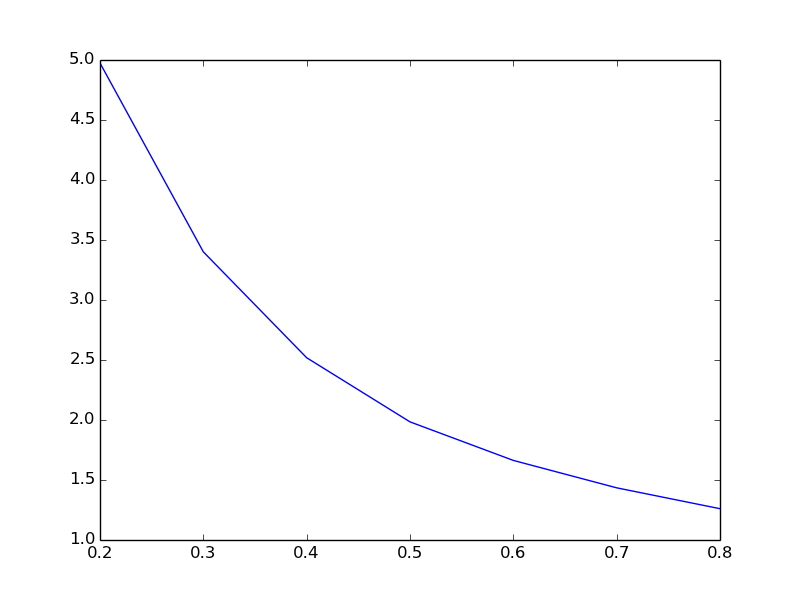
\includegraphics[width = 0.8\textwidth]{../results/exercise12}
 \caption{After convergence, the weight is adjusted such that applying $x_0$, $y = \omega$ and we observe that $\omega = \frac{1}{z}$, whereas $z$ is the probability of $x_0 = 1$}
 \label{fig:bild1}
\end{figure}

\subsection{Question 1.3}

We have a linear neuron $y = \omega * x$

\subsubsection{Show that $\Theta = \langle y^2 \rangle_x = z * y_0^2$}

\begin{align*}
	\Theta(t) = \frac{1}{\tau} * \int_{-\infty}^{t} y^p (s)\exp(-\frac{t-s}{\tau}) \mathrm{d}s \\
	\Theta(t) \approx \langle y^p \rangle_t \approx \langle y^p \rangle_x \\
	\Theta(t) = \frac{1}{\tau} * y^2 \int_{-\infty}^t exp(-\frac{t-s}{\tau}) \mathrm{d}s \\
	\Theta(t) = \frac{1}{\tau} * y^2 * \big{[} \frac{\tau}{s} * \exp(-\frac{t-s}{\tau}) \big{]_{-\infty}^t} \\
	\Theta(t) = \frac{1}{t} * y^2 = \langle y^2 \rangle = \langle (\omega * x)^2 \rangle
\end{align*}

When applying an input $x_0$ with a probability of $z$, then the average at the output is $z * y_0$ where $y_0 = \omega * x_0$, as we can see in the last equation.

\subsubsection{Show that $\langle \frac{\mathrm{d}\omega}{\mathrm{d}t} \rangle = \eta * z * x_0 * y_0^2 * (1 - z * y_0)$}

\begin{align*}
	\frac{\mathrm{d}\omega}{\mathrm{d}t} = \eta * x * (y^2 - y * \Theta) \\
	\langle \frac{\mathrm{d}\omega}{\mathrm{d}t} \rangle = \langle \eta * x * (y^2 - y * \Theta) \rangle \\
	\langle \frac{\mathrm{d}\omega}{\mathrm{d}t} \rangle = \eta * \langle x * (y^2 - y * z * y_0^2) \rangle \\
	\langle \frac{\mathrm{d}\omega}{\mathrm{d}t} \rangle = = \eta * z * x_0 * y_0^2 * (1- z * y_0) \\
\end{align*}

\section{Question 2}

\subsection{Question 2.1}

\begin{align*}
	F(\omega) = \langle (\frac{y}{\sigma_y})^3 \rangle \\
	\frac{\mathrm{d}F}{\mathrm{d}\omega}(\omega) = \langle \frac{\mathrm{d}{\mathrm{d}\omega}}(\frac{y}{\sigma_y})^3 \rangle \\
	= \langle 3 * (\frac{y}{\sigma_y})^2 * \frac{\frac{\mathrm{d}y}{\mathrm{d}\omega}*\sigma_y - y * \frac{\mathrm{d}}{\mathrm{d}*\omega}\sigma_y}{\sigma_y^2} \rangle \\
	= \langle 3 * (\frac{y^2}{\langle y^2 \rangle}) * \frac{x* \sigma_y - y * \frac{1}{\sigma_y} * \langle 2 * y * x \rangle}{\sigma_y^2} \rangle \\
	= \langle \frac{3 * y^2 * x}{\sigma_y^3} - \frac{3 * y^3 * \langle y * x \rangle}{\sigma_y^5} \rangle \\
	= \langle \frac{3 * y^2 * x}{\sigma_y^3} \rangle - \frac{\langle y^3 \rangle}{\langle y^2 \rangle} * \frac{\langle y * x \rangle}{\sigma_y^3} \\
\end{align*}
$\Theta$ is equal to $\frac{\langle y^3 \rangle}{\langle y^2 \rangle}$, therefore we can write:

\begin{align*}
	= \frac{3}{\sigma_y^3} * \langle y^2 * x \rangle - \Theta * \langle x * y \rangle \\
	= \frac{3}{\sigma_y^3} * \frac{1}{n} * \sum_{i}^{n} y^2*x - \Theta * \frac{1}{n} * \sum_{i}^{n} x * y \\
\end{align*}
This is the batch rule. We can transform this to an online rule:
\begin{align*}
	= \frac{3}{\sigma_y^3} * y^2*x - \Theta * x * y
\end{align*}
From which we ca dedude that $\frac{\mathrm{d}F}{\mathrm{d}\omega} \propto x y^2 - x y\Theta$

\subsection{Question 2.2}

\begin{figure}[H]
 \centering
 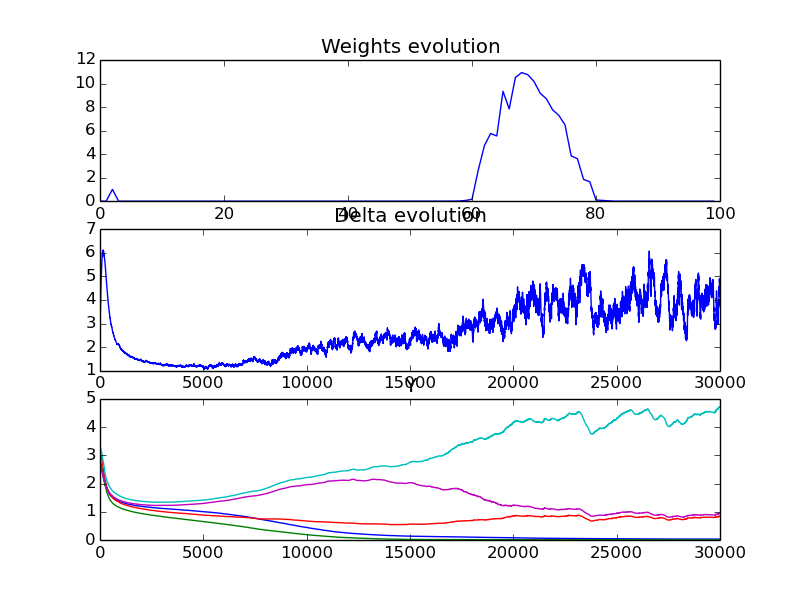
\includegraphics[width = 0.8\textwidth]{../results/exercise222}
 \caption{}
 \label{fig:bild1}
\end{figure}

\subsection{Question 2.3}


\section{Question 3}

Figure \ref{bil4} and \ref{bild3} are two examples of a receptive field formation in a BCM neuron. In both examples, it is clearly visible to which of the pixels the neuron is specialized.

More discussion needed...

\begin{figure}[H]
 \centering
 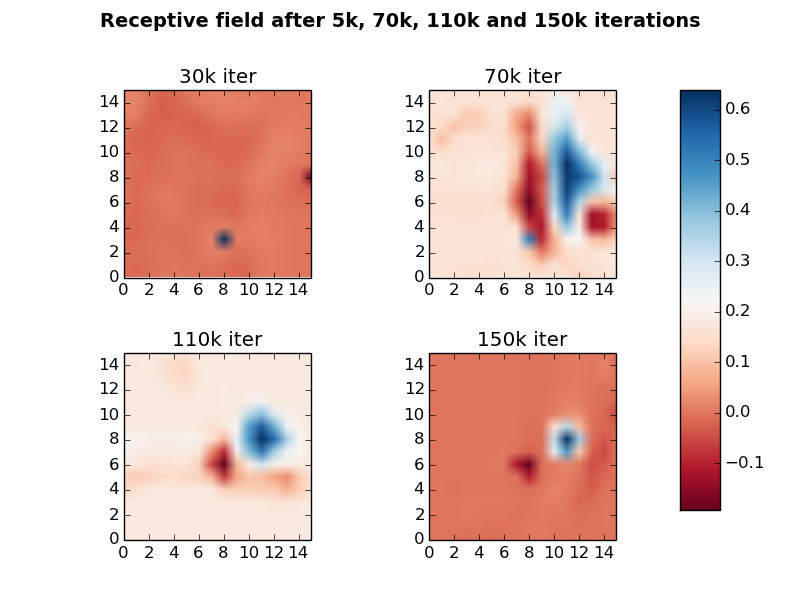
\includegraphics[width = 0.8\textwidth]{../results/exercise3b}
 \caption{}
 \label{fig:bild3}
\end{figure}

\begin{figure}[H]
 \centering
 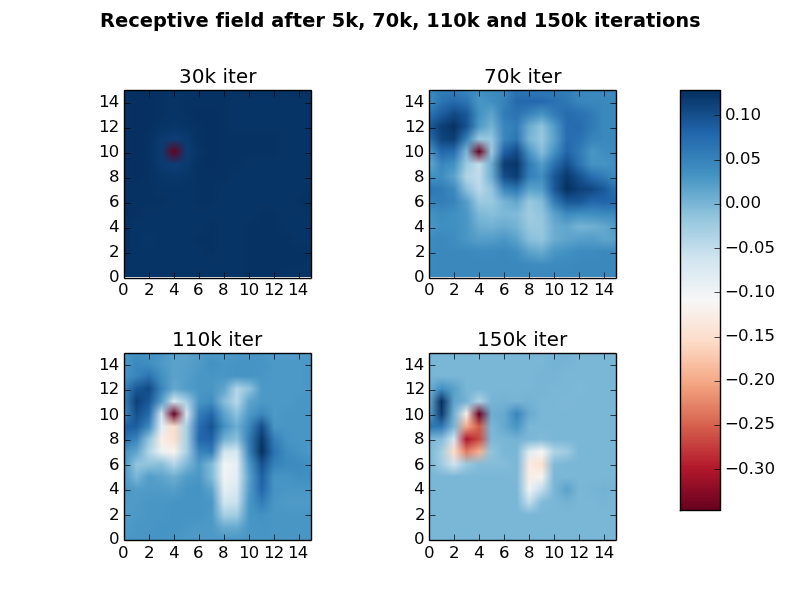
\includegraphics[width = 0.8\textwidth]{../results/exercise3c}
 \caption{}
 \label{fig:bild4}
\end{figure}


\end{document}